\documentclass[a4paper,twoside]{article}
\usepackage[T1]{fontenc}
\usepackage[utf8]{inputenc}
\usepackage{epsfig}
\usepackage{subcaption}
\usepackage{calc}
\usepackage{amssymb}
\usepackage{amstext}
\usepackage{amsmath}
\usepackage{amsthm}
\usepackage{multicol}
\usepackage{pslatex}
\usepackage{apalike}
\usepackage{algorithm2e}
\usepackage[bottom]{footmisc}
\usepackage{booktabs}
\usepackage{url}
\usepackage[hidelinks,pdfauthor={},pdftitle={Inspectable Narrative Graphs: Evidence-Linked Extraction and Contextual Selection},pdfcreator={LaTeX},pdfsubject={Anonymous position paper}]{hyperref}
\usepackage{SCITEPRESS}
\newcommand{\Temperature}{0.7}
\newcommand{\TopP}{0.8}
\newcommand{\TopK}{20}
\newcommand{\Seed}{1988649846}
\newcommand{\OutputTokens}{2,048}
\newcommand{\ContextTokens}{12,288}
\newcommand{\StorySentences}{14}
\newcommand{\FableWords}{133}
\newcommand{\AliceWords}{112}
\newcommand{\HolmesWords}{159}
\newcommand{\CompactCalls}{12}
\newcommand{\ProseCalls}{9}
\newcommand{\ProseParsed}{7}
\newcommand{\IntervalsKept}{79}
\newcommand{\IntervalsEligible}{79}
\newcommand{\OrchardLocationRecall}{0.750}
\newcommand{\MainCalls}{21}
\newcommand{\MainAllocation}{454.82}
\newcommand{\CompactAllocation}{249.45}
\newcommand{\ProseAllocation}{205.37}
\newcommand{\CompactRequest}{104.72}
\newcommand{\ProseRequest}{57.24}
\newcommand{\FableAFone}{0.625}
\newcommand{\FableACoverage}{6 of 8}
\newcommand{\FableBFone}{0.308}
\newcommand{\FableBCoverage}{4 of 8}
\newcommand{\AliceAFone}{0.000}
\newcommand{\AliceACoverage}{1 of 4}
\newcommand{\AliceBFone}{0.000}
\newcommand{\AliceBCoverage}{3 of 4}
\newcommand{\FableQuestion}{Which physical running/waking, capture, binding, rope-gnawing and release relationships involve the Lion, Mouse, hunters and ropes? Exclude dialogue, intentions, laughter and the moral.}
\newcommand{\HarborQuestion}{Which directly narrated location relationships have an explicitly stated interval overlapping day 2 up to but not including day 4? Return all of them with their full evidence-stated intervals, not clipped to the question window. Exclude undated locations and beliefs.}
\newcommand{\AliceActionQuestion}{Which sitting/location, reading/inspection and running relationships involve Alice, her sister, the book, bank and Rabbit? Exclude thoughts, feelings, appearance and book-content properties.}
\newcommand{\AliceClaimQuestion}{What does the passage say about the book's absent content and Alice's thoughts about the usefulness of such books and making a daisy-chain? Exclude physical actions, locations, appearance and the Rabbit; preserve questions and consideration without treating them as decisions.}

% Conference-native artwork: figures are NOT scaled-down general-paper plates.
\newcommand{\FableFigure}{
\begin{figure*}[!t]
\centering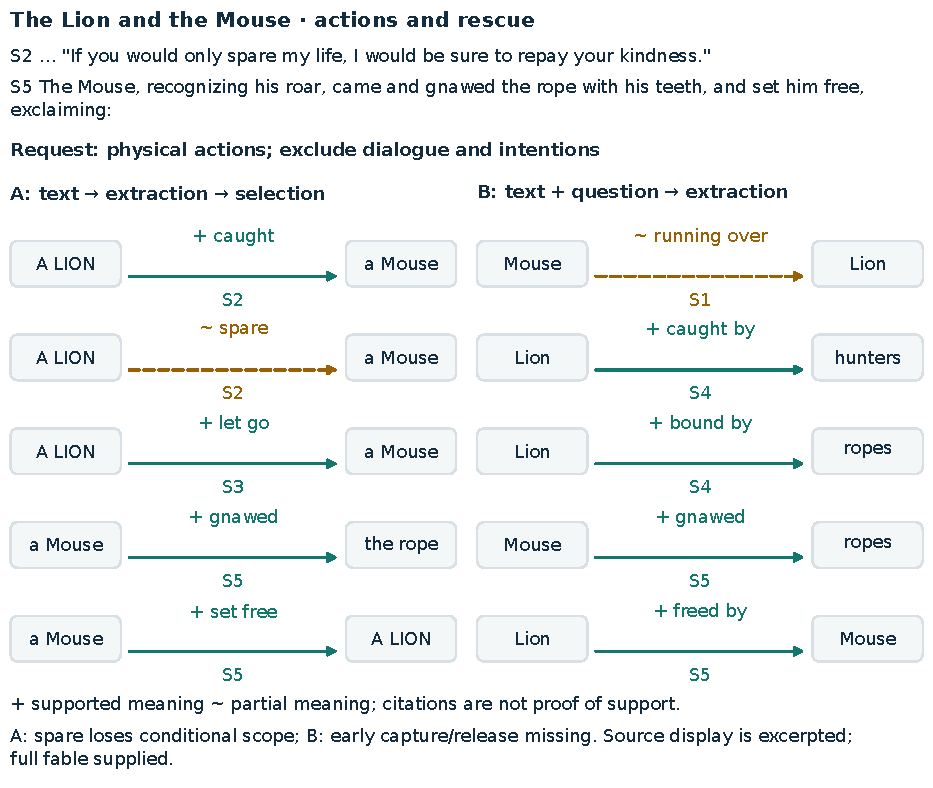
\includegraphics[width=\textwidth]{figures/fable.pdf}
\caption{Fable actions from pre-extract/select (A) and independent contextual extraction (B). + indicates supported meaning and $\sim$ partial meaning. Display: five of eight A records and all five B records. A's awakening, hunter capture and rope binding are omitted only from display. All predictions remain scored. Executed question: \FableQuestion\ Source display excerpts S2 and S5 from the complete supplied fable. The spare edge loses conditional scope and retains the misspelled key \texttt{valid until}. B loses the face-specific running endpoint and omits the early capture/release. Other displayed qualifications are null. Assessments are Codex-authored.}
\label{fig:fable}
\end{figure*}}
\newcommand{\HarborFigure}{
\begin{figure*}[!t]
\centering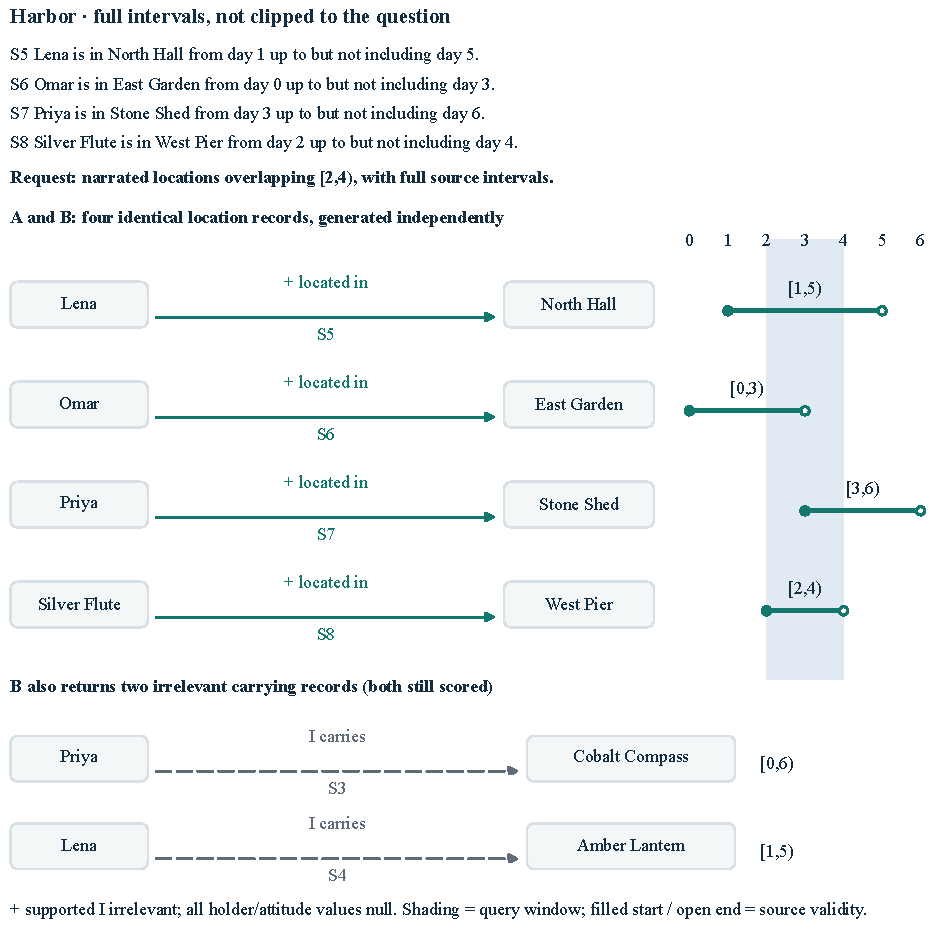
\includegraphics[width=\textwidth]{figures/harbor.pdf}
\caption{Harbor locations from pre-extract/select (A) and contextual extraction (B). Four independently generated records coincide and are shown in aligned rows. B also returns the two carrying edges below. Filled/open circles mark included/excluded bounds. Shading shows the query window, not rewritten validity. Executed question: \HarborQuestion\ Source display S5--S8 from the fourteen sentences supplied to both approaches. All six B predictions remain scored. + indicates supported meaning and I supported but irrelevant content. Holder and attitude are null throughout.}
\label{fig:harbor}
\end{figure*}}
\newcommand{\AliceFigure}{
\begin{figure*}[!t]
\centering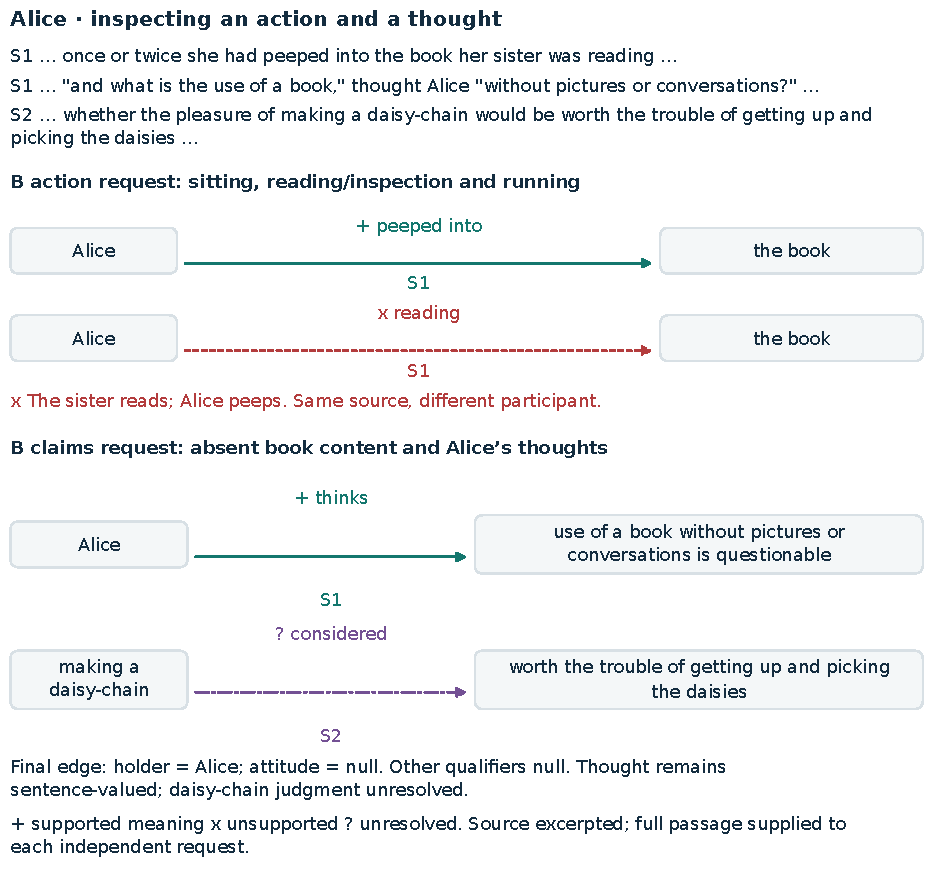
\includegraphics[width=\textwidth]{figures/alice.pdf}
\caption{Alice: independent contextual extraction (B) for two requests over identical complete evidence. Display: two of five action edges (two sitting edges and Rabbit running omitted) and two of three claims (book content omitted). All remain scored. Executed action question: \AliceActionQuestion\ Executed claims question: \AliceClaimQuestion\ Source excerpts are marked. + indicates supported meaning, x an unsupported participant, and ? unresolved consideration. The thought remains the actual sentence-valued object. All bounds are null. The final record has holder Alice and null attitude.}
\label{fig:alice}
\end{figure*}}

\begin{document}
\title{Contextual Ontology Extraction and Inspection of Temporal Narrative Networks}
\author{}
\keywords{Natural Language Processing, Knowledge Representation and Reasoning, Large Language Models, Visualization.}
\abstract{We present a narrative extraction workflow connecting readers' questions, generated relationships, temporal and attribution details, and visual inspection of evidence and errors. We compare extraction before seeing a question followed by fixed selection with independent contextual extraction on three synthetic stories and three short published passages. Assessment separates strict agreement with reference answers from preserved meaning, relevance and unresolved interpretation. All \CompactCalls\ story responses were parseable. Fixed selection matched every possession and dated location target without extras, whereas contextual answers retained irrelevant facts. On fable actions, strict F1 was \FableAFone\ for selection and \FableBFone\ for contextual extraction. Query-guided extraction of statements and thoughts from an excerpt of Alice’s Adventures in Wonderland preserved \AliceBCoverage\ semantic targets despite zero strict F1. Prose parsing succeeded in \ProseParsed\ of \ProseCalls\ calls. The workflow makes these mixed results  easy to inspect, including useful thought representations, incorrect participants and lost conditional scope. These small development comparisons identify concrete extraction and selection problems for further research. }
\onecolumn\maketitle\normalsize\setcounter{footnote}{0}\vfill

\section{\uppercase{Introduction}}
\noindent Stories describe people, places and objects whose relationships change over time. Readers may want to know who carries an object, where it is, or what a character believes about it. We present a workflow for exploring narrative ontologies, structured representations of a story's entities and relationships, as temporal networks. Nodes represent characters, objects or places, and edges show their relationships. Temporal details indicate when a relationship holds, while links to the text let readers check its basis. Readers can also examine whether a relationship reflects a character's belief or the narrator's account.

We compare two ways to produce a network for a reader's question. \emph{Pre-extract/select} (A) first extracts relationships without seeing the question, then selects existing records using fixed filters. \emph{Contextual extraction} (B) extracts relationships directly from the same text with the question supplied. Both use records with entity names, evidence citations, time intervals and attribution. Our contributions are:

\begin{enumerate}
\item An implemented workflow connecting narrative questions, temporal networks and source evidence. Linked views let readers inspect relationships and trace their meaning to the text (Section~3 and Figures~\ref{fig:orchard}-\ref{fig:alice}).
\item An empirical comparison of extraction before and after the question is supplied. Results on synthetic stories and published prose help distinguish problems in extracting relationships from problems in selecting relevant ones (Section~5).
\item An assessment combining agreement with reference answers, preservation of meaning, relevance and unresolved interpretation. Tables~\ref{tab:compact} and~\ref{tab:prose} and the annotated networks show useful partial results alongside errors.
\end{enumerate}

Together, these contributions support the inspection of narrative ontologies beyond a single accuracy score. Small development comparisons show which relationships survive extraction, which details are lost, and how questions affect the resulting networks.

\OrchardFigure
\section{\uppercase{Related Work}}
\noindent \emph{Extraction and representation.} TextRunner extracts relationships without a predefined relation vocabulary and indexes them for later queries \cite{banko2007}. SPIRES uses recursive language model prompts to fill a supplied schema and link entities to external vocabularies \cite{caufield2024}. Building on these approaches, we compare extraction with and without an available question while retaining local entity names and supporting text.

Temporal ontologies provide a foundation for describing change. OWL-Time represents instants, intervals, durations and ordering \cite{time2017}. GRaSP connects statements, textual mentions, sources and attitudes, with an interface linking events to their evidence \cite{fokkens2017}. These foundations inform our compact representation of when relationships hold and who expresses a belief.

\emph{Comparison and inspection.} RelVis combines extraction comparison, visual inspection and error annotation \cite{schneider2017}. It also distinguishes valid relationships missing from reference annotations from extraction errors. CaRB improves reference annotations and scoring through partial coverage and checks on the alignment of relationships and their participants \cite{bhardwaj2019}. Using our own strict matcher, we report agreement separately from judgments about preserved meaning, missing details and unresolved readings.

Our visualization draws on established filtering, linked selection and coordinated views \cite{heer2012}. The contribution brings these ideas together for narrative questions, preserving temporal information and attribution while comparing when extraction occurs relative to the question. Worked examples reveal both useful relationships and errors, such as a correct action linked to the wrong participant. The cited systems provide methodological foundations rather than experimental baselines.



\section{\uppercase{Representation and Methods}}


\subsection{Evidence and Qualified Records}
\noindent Each request receives the complete selected story or contiguous excerpt with unchanged wording and numbered evidence spans. Each extracted relationship is represented by a qualified record:
\begin{equation}
\label{eq:qualified-record}
f = \langle s, r, o, E, t_0, t_1, h, a \rangle .
\end{equation}
The subject $s$, relation $r$ and object $o$ define a network edge. Its remaining fields provide evidence identifiers $E$, temporal bounds $t_0$ and $t_1$, and attribution through a holder $h$ and attitude $a$. The model supplies every record value. The runtime never fills missing meaning from reference answers.

The following illustration is authored to explain the format and is not a model result:
\begin{small}\begin{verbatim}
{"subject":"Nara", "relation":"carries",
 "object":"map", "evidence_ids":["X1"],
 "valid_from":2, "valid_until":5,
 "holder":null, "attitude":null}
\end{verbatim}\end{small}
Given supporting evidence in span \texttt{X1}, this record states that Nara carries the map during $[2,5)$, including the start and excluding the end. A query window $[3,4)$ selects the overlapping record while preserving its original bounds.

Temporal bounds describe intrinsic validity, meaning when the relationship holds. An occurrence or observation alone does not establish its onset or duration. Unsupported bounds remain \texttt{null}, indicating unspecified information rather than timeless validity or falsehood. Relative phrases such as ``shortly after'' are not converted into numbers, so their temporal detail may remain unrepresented in these bounds.
For belief, $(s,r,o)$ describes the believed relationship, $h$ names the believer and $a=\texttt{believes}$. Direct narration uses \texttt{null} for both attribution fields without implying that a character knows the stated relationship. Speech and mental acts may also be explicit relationships, without treating their content as established reality.
Pronoun resolution requires a clear referent in the excerpt. The frozen matcher treats missing nullable fields as unspecified, while the field-compliance assessment separately records their absence.



\subsection{Extraction Before or With the Question}
\noindent Pre-extract/select (A) first requests all explicitly supported relationships without showing the questions. Its actual output is frozen before any contextual request is sent. CPU selection retains existing records by relation category, requested entity, attribution status or explicit interval overlap. Synthetic rules distinguish possession, dated location and belief/narration. Prose rules use lexical action and claim categories appropriate to each passage. These fixed rules do not infer relationships, repair meanings or consult reference answers.

Contextual extraction (B) receives the same complete evidence and one question, requesting only relationships needed to answer it. It never consumes A's graph. Both approaches share the representation, model and authoring conventions. Prompts, questions, selectors and call order are frozen before each batch. All extractions without questions precede contextual transmission. Each request runs once without adaptive repair, independently of another output's failure.

The experiments use \texttt{Qwen/Qwen3-8B-AWQ} in nonthinking mode \cite{qwen2025,qwenmodel}, served by vLLM \cite{kwon2023} on one RTX 4090. Temperature is \Temperature, top-p \TopP, top-k \TopK, and seed \Seed.  Ordinary JSON is requested without a guided schema. 



\subsection{Inspecting Actual Output}
\noindent Graph edges retain generated direction, names, citations and qualifications. Only identical endpoint strings share a display identity. Aliases are not inferred, and objects containing sentences remain literal nodes. The Orchard network makes shared participants and connectivity visible (Figure~\ref{fig:orchard}). Node fills denote display categories, not model types or correctness. Status symbols and edge styles distinguish supported, partial, unsupported, unresolved and irrelevant content. A citation highlight is a navigation aid, not verification. Other figures use relationship rows for long labels. Missing targets appear beside graphs, never as corrected model edges. Display subsets do not change scoring denominators.
\FableFigure





\section{\uppercase{Evaluation}}




\subsection{Materials and Annotation}
\noindent Each evaluation case combines a numbered narrative $T_i$, a reader's question $q_{ij}$ and reference records $\mathcal{R}_{ij}$, including accepted alternatives:
\begin{equation}
\label{eq:evaluation-case}
d_{ij} = \langle T_i, q_{ij}, \mathcal{R}_{ij} \rangle .
\end{equation}
Evidence, question scope, reference alternatives and normalization rules are frozen before generation, giving both approaches the same evaluation target.

The controlled stories Harbor, Orchard and Museum each contain \StorySentences\ evidence sentences. Three questions address possession, location within an interval, and belief versus narration. These tasks reveal whether extracted networks preserve relationships together with their temporal and attribution details. Harbor and Orchard informed development. Museum varies sentence order and entity relationships fixed before this batch. Earlier experiments remain separate.

The prose comparison uses Townsend's complete Lion and Mouse fable (\FableWords\ words), the opening of \emph{Alice's Adventures in Wonderland} (\AliceWords\ words), and a contiguous opening passage from \emph{The Red-Headed League} (\HolmesWords\ words) \cite{aesop,carroll,doyle}. Citations identify the retained Gutenberg editions. Passages were selected before execution for identifiable participants, actions, thoughts and dialogue, with two questions per passage addressing actions and claims.

RelVis demonstrates the value of inspecting extraction errors, while CaRB shows how reference annotations and matching choices affect evaluation \cite{schneider2017,bhardwaj2019}. Building on these findings, our design connects extraction before or after question disclosure to the preservation of relevance, temporal bounds and attribution in narrative networks.

Synthetic inventories distinguish unsupported relationships from supported but irrelevant ones. Prose references cover the requested information. Separate semantic assessments distinguish wording differences from lost or altered meaning. Reference answers and response assessments have not undergone independent human validation. Ambiguous interpretations, including Holmes's vocative and Alice's daisy-chain consideration, remain open to author review.




\subsection{Agreement, Meaning and Failure}
\noindent \emph{Strict qualified-fact matching} requires agreement on the normalized relationship, evidence set, temporal bounds and attribution. Let $n$ be the number of predictions, $m$ the number of reference targets and $k$ the number of one-to-one matches against frozen alternatives. For nonzero denominators,
\begin{equation}
\label{eq:strict-scores}
P=\frac{k}{n}, \qquad
R=\frac{k}{m}, \qquad
F_1=\frac{2k}{n+m}.
\end{equation}
Incorrect, duplicate, irrelevant and unresolved predictions remain in $n$, while omissions reduce recall. Bare relationship scores ignore citations and qualifications. Strict F1 therefore measures reference agreement, not factual truth.

Semantic assessment separately labels supported, partially supported, unsupported and unresolved content, alongside qualification errors and relevance. Target coverage counts distinct meanings explicitly preserved. One prediction may cover several targets, but partial support is not full coverage. Support requires positive evidence. Missing meaning is never supplied, and equivalence rules remain unchanged after generation.

Strict parsing rejects malformed JSON, duplicate keys and non-JSON constants. A separately recorded recovery may remove only trailing commas immediately before closing delimiters outside strings, preserving raw bytes and an edit record. Neither main batch required recovery. Unparseable outputs have unavailable graph scores and are not scored as intentionally empty graphs.

The analysis is descriptive. These purposively selected development examples share stories and reuse outputs during selection. Records therefore cannot be treated as independent experimental trials, and no significance tests are applied.

\AliceFigure






\section{\uppercase{Results}}

\subsection{Synthetic Selection and Qualifications}
\noindent All \CompactCalls\ compact-story outputs are strictly parseable. Pre-extract/select (A) matches every possession and dated location target without extras (Table~\ref{tab:compact}). Contextual extraction (B) commonly retrieves the requested physical relationships but returns irrelevant facts in every answer. Orchard's location answer also omits a target: recall is \OrchardLocationRecall. The fresh Museum story shows the same excessive selection as the earlier stories.

\begin{table*}[t]
% Positive inset keeps the top caption within the nominal text margin.
\vspace*{6pt}
\caption{Compact-story v2 strict qualified-fact scores. A: pre-extract/select. B: contextual extraction. $n$ includes every prediction. Targets per story: possession 5, location 4, belief/reality 4. No historical recoveries are pooled.}\label{tab:compact}
\centering\small
\begin{tabular}{llrrrrrrrr}\toprule
Story & Question & $n_A$ & $P_A$ & $R_A$ & $F1_A$ & $n_B$ & $P_B$ & $R_B$ & $F1_B$\\\midrule
Harbor & Possession & 5 & 1.000 & 1.000 & 1.000 & 10 & 0.500 & 1.000 & 0.667 \\
Harbor & Location & 4 & 1.000 & 1.000 & 1.000 & 6 & 0.667 & 1.000 & 0.800 \\
Harbor & Belief/reality & 5 & 0.000 & 0.000 & 0.000 & 14 & 0.143 & 0.500 & 0.222 \\
Orchard & Possession & 5 & 1.000 & 1.000 & 1.000 & 12 & 0.417 & 1.000 & 0.588 \\
Orchard & Location & 4 & 1.000 & 1.000 & 1.000 & 5 & 0.600 & 0.750 & 0.667 \\
Orchard & Belief/reality & 4 & 1.000 & 1.000 & 1.000 & 13 & 0.154 & 0.500 & 0.235 \\
Museum & Possession & 5 & 1.000 & 1.000 & 1.000 & 13 & 0.385 & 1.000 & 0.556 \\
Museum & Location & 4 & 1.000 & 1.000 & 1.000 & 5 & 0.800 & 1.000 & 0.889 \\
Museum & Belief/reality & 4 & 0.000 & 0.000 & 0.000 & 14 & 0.143 & 0.500 & 0.222 \\\bottomrule\end{tabular}\end{table*}


Orchard illustrates actual selection from a broader model extraction (Figure~\ref{fig:orchard}). Its five ownership/carrying records connect six nodes, retaining explicit carrying intervals. This illustration does not establish a construction effect. The companion contrasts this slice with the twelve-record contextual answer, which also retains seven irrelevant locations.

Among emitted records with identifiable explicitly timed sources, \IntervalsKept\ of \IntervalsEligible\ preserve their full intervals, including irrelevant records. This is conditional preservation, not temporal recall over every reference. The companion's Harbor timeline distinguishes these intervals from the query window. Attribution is less stable: Orchard's pre-extraction decomposes beliefs correctly, whereas Harbor and Museum use sentence-valued belief objects that disrupt selection.




\subsection{Published Prose and Partial Meaning}
\noindent The prose comparison yields \ProseParsed\ strictly parseable responses from \ProseCalls\ calls. Extra closing braces invalidate Holmes's pre-extraction and contextual action answer. The shared pre-extraction failure blocks both A questions (Table~\ref{tab:prose}). The parseable Holmes claims answer contains partial and unresolved content without fully covered targets.

\begin{table*}[t]
\caption{Published prose: strict qualified-fact precision, recall and F1, separate from Codex-authored semantic support (S), partial support (P), unsupported (X), unresolved (U), and semantic target coverage. NA = unavailable due to parse failure, not an empty graph. All parseable predictions have valid evidence IDs; that does not establish support.}\label{tab:prose}
\centering\small\begin{tabular}{lllrrrrrr}\toprule
Passage & Question & Method & $n$ & Precision & Recall & F1 & S/P/X/U & Coverage\\\midrule
Alice & Actions & A & 2 & 0.500 & 0.200 & 0.286 & 2/0/0/0 & 3/5 \\
Alice & Actions & B & 5 & 0.400 & 0.400 & 0.400 & 3/1/1/0 & 3/5 \\
Alice & Claims & A & 4 & 0.000 & 0.000 & 0.000 & 2/2/0/0 & 1/4 \\
Alice & Claims & B & 3 & 0.000 & 0.000 & 0.000 & 2/0/0/1 & 3/4 \\
Fable & Actions & A & 8 & 0.625 & 0.625 & 0.625 & 6/1/0/1 & 6/8 \\
Fable & Actions & B & 5 & 0.400 & 0.250 & 0.308 & 4/1/0/0 & 4/8 \\
Fable & Claims & A & 1 & 0.000 & 0.000 & 0.000 & 1/0/0/0 & 2/5 \\
Fable & Claims & B & 4 & 0.000 & 0.000 & 0.000 & 1/3/0/0 & 0/5 \\
Holmes & Actions & A & NA & NA & NA & NA & NA & NA \\
Holmes & Actions & B & NA & NA & NA & NA & NA & NA \\
Holmes & Claims & A & NA & NA & NA & NA & NA & NA \\
Holmes & Claims & B & 3 & 0.000 & 0.000 & 0.000 & 0/1/0/2 & 0/5 \\\bottomrule\end{tabular}\end{table*}


For fable actions, pre-extract/select performs better on both measures, with strict F1 \FableAFone\ versus \FableBFone\ and semantic coverage \FableACoverage\ versus \FableBCoverage. A therefore preserves most target action meanings. Both approaches recover the later rescue, but contextual extraction omits the early capture and release. A's \texttt{spare} relation loses the scope of the Mouse's conditional plea, while some supported passive formulations fail strict matching (Figure~\ref{fig:fable}). These networks capture useful narrative content despite incomplete agreement.

In the Alice excerpt, contextual extraction improves semantic coverage from \AliceACoverage\ to \AliceBCoverage, although both strict F1 scores remain zero. Its combined thought statement preserves rhetorical meaning without the requested decomposition. Contextual extraction also incorrectly assigns reading to Alice instead of her sister. Whether the daisy-chain record converts considering an action's worth into judging it worthwhile remains unresolved (Figure~\ref{fig:alice}). The improvement is therefore in retained meaning, with participant errors and interpretive uncertainty still visible.









\section{\uppercase{Discussion and Limitations}}

\noindent This work advances narrative ontology development through an implemented model connecting reader intent, temporal scope and evidence inspection. It makes the construction of a narrative network an explicit part of answering a question, with relationships represented together with the information needed to interpret and verify them.
Building on relation extraction \cite{banko2007}, temporal and perspective representation \cite{time2017,fokkens2017}, and visual error analysis \cite{schneider2017}, the contribution is a shared framework for comparing how question availability affects extraction and selection. Relevance and interval filters provide a mechanism for reducing displayed graph size while retaining source evidence and original temporal bounds. Contextual generation explores the complementary possibility of focusing relationships during extraction itself.

The examples demonstrate useful preservation of narrative structure. Pre-extraction captures most annotated fable actions, contextual extraction increases semantic coverage in Alice, and Harbor retains explicit intervals. These findings establish concrete capabilities on which further ontology development can build. The framework also connects participant errors, lost conditions and irrelevant relationships to their source passages, making improvements in parsing and selection directly assessable. Its value lies in combining usable partial networks with an explicit account of what they preserve and omit.




\section{\uppercase{Conclusion}}
\noindent We present a workflow connecting narrative questions, qualified relationships and evidence inspection. Comparing pre-extract/select with contextual extraction reveals useful action and thought information alongside relevance and participant errors. Selection performs better on several questions, while contextual extraction preserves more of Alice's claims. Combining strict agreement, semantic assessment and visualization provides a concrete basis for improving narrative extraction and studying its use.

\section{\uppercase{AI Use and Annotation Provenance}}
\label{sec:disclosure}
\noindent OpenAI Codex \cite{openai2025} assisted implementation of code. Qwen generated the simulated user prompt exchange for query ontological searches.

\bibliographystyle{apalike}
{\small\bibliography{references}}
\section*{APPENDIX}
\noindent Qwen3-8B-AWQ revision: \texttt{4da05a8edb55c6046cce9585}\allowbreak\texttt{86c33b61da07bb79}. Software: vLLM 0.10.2, Transformers 4.55.2. The pinned template uses \texttt{enable\_thinking=False}. The concise companion indexes complete machine-readable requests, outputs, reference alternatives and assessments.
\end{document}
